\documentclass{standalone}
\usepackage{tikz}
\usetikzlibrary{shapes.geometric}

\begin{document}

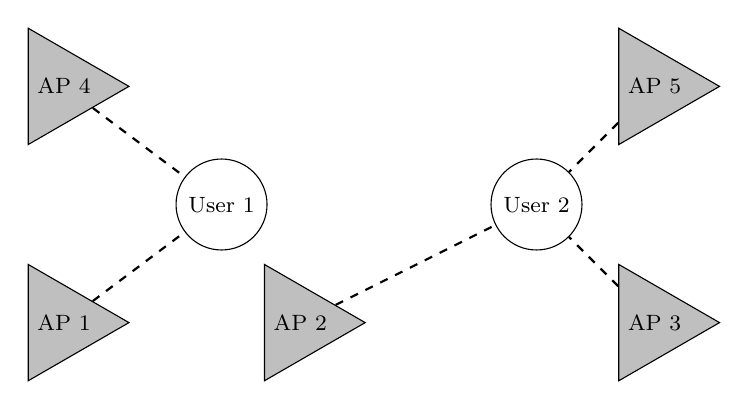
\begin{tikzpicture}[font=\footnotesize,
    AP/.style={isosceles triangle, isosceles triangle apex angle=60, draw, fill=gray!50},
    User/.style={draw, circle, fill=white, minimum size=1.2em},
    Line/.style={-, dashed, thick}]
    
    % Drawing Access Points
    \node[AP]     (AP1)  at (-3,0) {AP 1};
    \node[AP]     (AP2)  at (0,0)  {AP 2};
    \node[AP]     (AP3)  at (4.5,0) {AP 3};
    \node[AP]     (AP4)  at (-3,3) {AP 4};
    \node[AP]     (AP5)  at (4.5,3) {AP 5};
    
    % Drawing Users
    \node[User]   (User1) at (-1,1.5) {User 1};
    \node[User]   (User2) at (3,1.5)  {User 2};
    
    % Connecting Access Points to Users with Dashed Lines
    \draw[Line] (AP1) -- (User1);
    \draw[Line] (AP4) -- (User1);
    \draw[Line] (AP2) -- (User2);
    \draw[Line] (AP3) -- (User2);
    \draw[Line] (AP5) -- (User2);
    
\end{tikzpicture}

\end{document}